\documentclass[12pt]{article}
%\usepackage{xltxtra}
\usepackage{fancyhdr}
\usepackage{graphicx}
\usepackage{enumerate}
\usepackage{amsmath}
\usepackage{amssymb, bm}
\usepackage{subfigure}
\usepackage{hyperref}
\hypersetup{ %
	colorlinks=true,
    linkcolor=blue, %mydarkblue,
    citecolor=blue, %mydarkblue,
    filecolor=blue, %mydarkblue,
    urlcolor=blue, %mydarkblue,
} 
%\usepackage[utf8]{inputenc}
%\usepackage[T1]{fontenc}
%\usepackage{fontspec}
%\usepackage{xunicode}

\newcommand{\iid}{\stackrel{\text{iid}}{\sim}}
\newcommand{\eqInDist}{\stackrel{\text{d}}{=}}

\newcommand{\mysec}[1]{Section~\ref{sec:#1}}
\newcommand{\eq}[1]{Eq.~(\ref{eq:#1})}
\newcommand{\myfig}[1]{Figure~\ref{fig:#1}}

\newcommand{\BEAS}{\begin{eqnarray*}}
\newcommand{\EEAS}{\end{eqnarray*}}
\newcommand{\BEA}{\begin{eqnarray}}
\newcommand{\EEA}{\end{eqnarray}}
\newcommand{\BEQ}{\begin{equation}}
\newcommand{\EEQ}{\end{equation}}
\newcommand{\BIT}{\begin{itemize}}
\newcommand{\EIT}{\end{itemize}}
\newcommand{\BNUM}{\begin{enumerate}}
\newcommand{\ENUM}{\end{enumerate}}
\newcommand{\BA}{\begin{array}}
\newcommand{\EA}{\end{array}}
\newcommand{\diag}{\mathop{\rm diag}}
\newcommand{\var}{\mathop{\rm var}}
\newcommand{\mean}{\mathop{\rm mean}}
\newcommand{\Diag}{\mathop{\rm Diag}}

\newcommand{\nn}{\nonumber}
\newcommand{\half}{\frac{1}{2}}
\newcommand{\1}{{\bf 1}}
\newcommand{\st}{\text{ s.t.}}
\newcommand{\ie}{\text{ i.e.}}
\newcommand{\rb}{\mathbb{R}}
\newcommand{\cb}{\mathbb{C}}
\newcommand{\zb}{\mathbb{Z}}
\newcommand{\tr}{{\rm tr}}
\newcommand{\idm}{I}
\newcommand{\BlackBox}{\rule{1.5ex}{1.5ex}}  % end of proof
\newcommand{\indep}{\bot\!\!\!\bot}


\newenvironment{proof}{\par\noindent{\bf Proof\ }}{\hfill\BlackBox\\[2mm]}

\newtheorem{proposition}{Proposition}
\newtheorem{lemma}{Lemma}


% If your paper is accepted, change the options for the package
% aistats2e as follows:
%
%\usepackage[accepted]{aistats2e}
%
% This option will print headings for the title of your paper and
% headings for the authors names, plus a copyright note at the end of
% the first column of the first page.
\setlength{\parindent}{0cm}
%\ifMain
\addtolength{\oddsidemargin}{-2cm}
\addtolength{\evensidemargin}{-2cm}
\setlength{\textwidth}{17.78cm}
\addtolength{\topmargin}{-2.7cm}
\setlength{\textheight}{24.24cm}
%\else
\addtolength{\parskip}{5mm}
%\fi
\pagestyle{fancy}

\title{Hwk 3}
\author{Simon Lacoste-Julien}

\begin{document}
\fancyhead{}
\fancyfoot{}

\fancyhead[R]{
  \begin{tabular}[b]{l}
    Name: \hspace{3cm} \\
    Student id: \hspace{3cm} \\
  \end{tabular}
  %\vspace*{10\baselineskip}
}
\fancyhead[L]{
  \begin{tabular}[b]{l}
    IFT6269-A2020  \\
    Prof: Simon Lacoste-Julien \\
  \end{tabular}
  %\vspace*{10\baselineskip}
}
\fancyhead[C]{
  \begin{tabular}[b]{c}
    {\bf Hwk 3} \\
    Due date: Nov 3, 2020
  \end{tabular}
}

%\vspace{0.3cm}

%As usual, please hand in on paper form your derivations and answers to the questions. You can use any programming language for your source code (submitted on Studium as per the website instructions). All the requested figures should be printed on paper with clear titles that indicate what the figures represent.


\textbf{Note:} There are 10 bonus points in this assignment. The maximum number of points achievable for this assignment is 80; though you will be graded over 70. If you get more points than 70, they can compensate other assignments.

\begin{enumerate}

%--------------------
%    Question 1
%--------------------
\item {\bf DGM (5 points)}  \\
\begin{minipage}[b]{0.7\textwidth}
Consider the directed graphical model $G$ on the right. 
Write down the implied factorization for any joint distribution $p \in \mathcal{L}(G)$.
Is it true that $X \indep Y \mid T$ for any $p \in \mathcal{L}(G)$? Prove or disprove.
\end{minipage}
\begin{minipage}{0.3\textwidth}
\vspace{-10mm}
\hspace{0.6cm}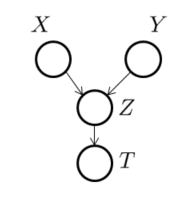
\includegraphics[scale=.5]{hwk3_GMex.png} \vspace{-10mm}
\end{minipage}

%--------------------
%    Question 2
%--------------------
\item {\bf D-separation in DGM (5 points)} \\
Indicate (yes or no) which conditional independence statements are true?
\begin{center}
\vspace{-0.2cm} 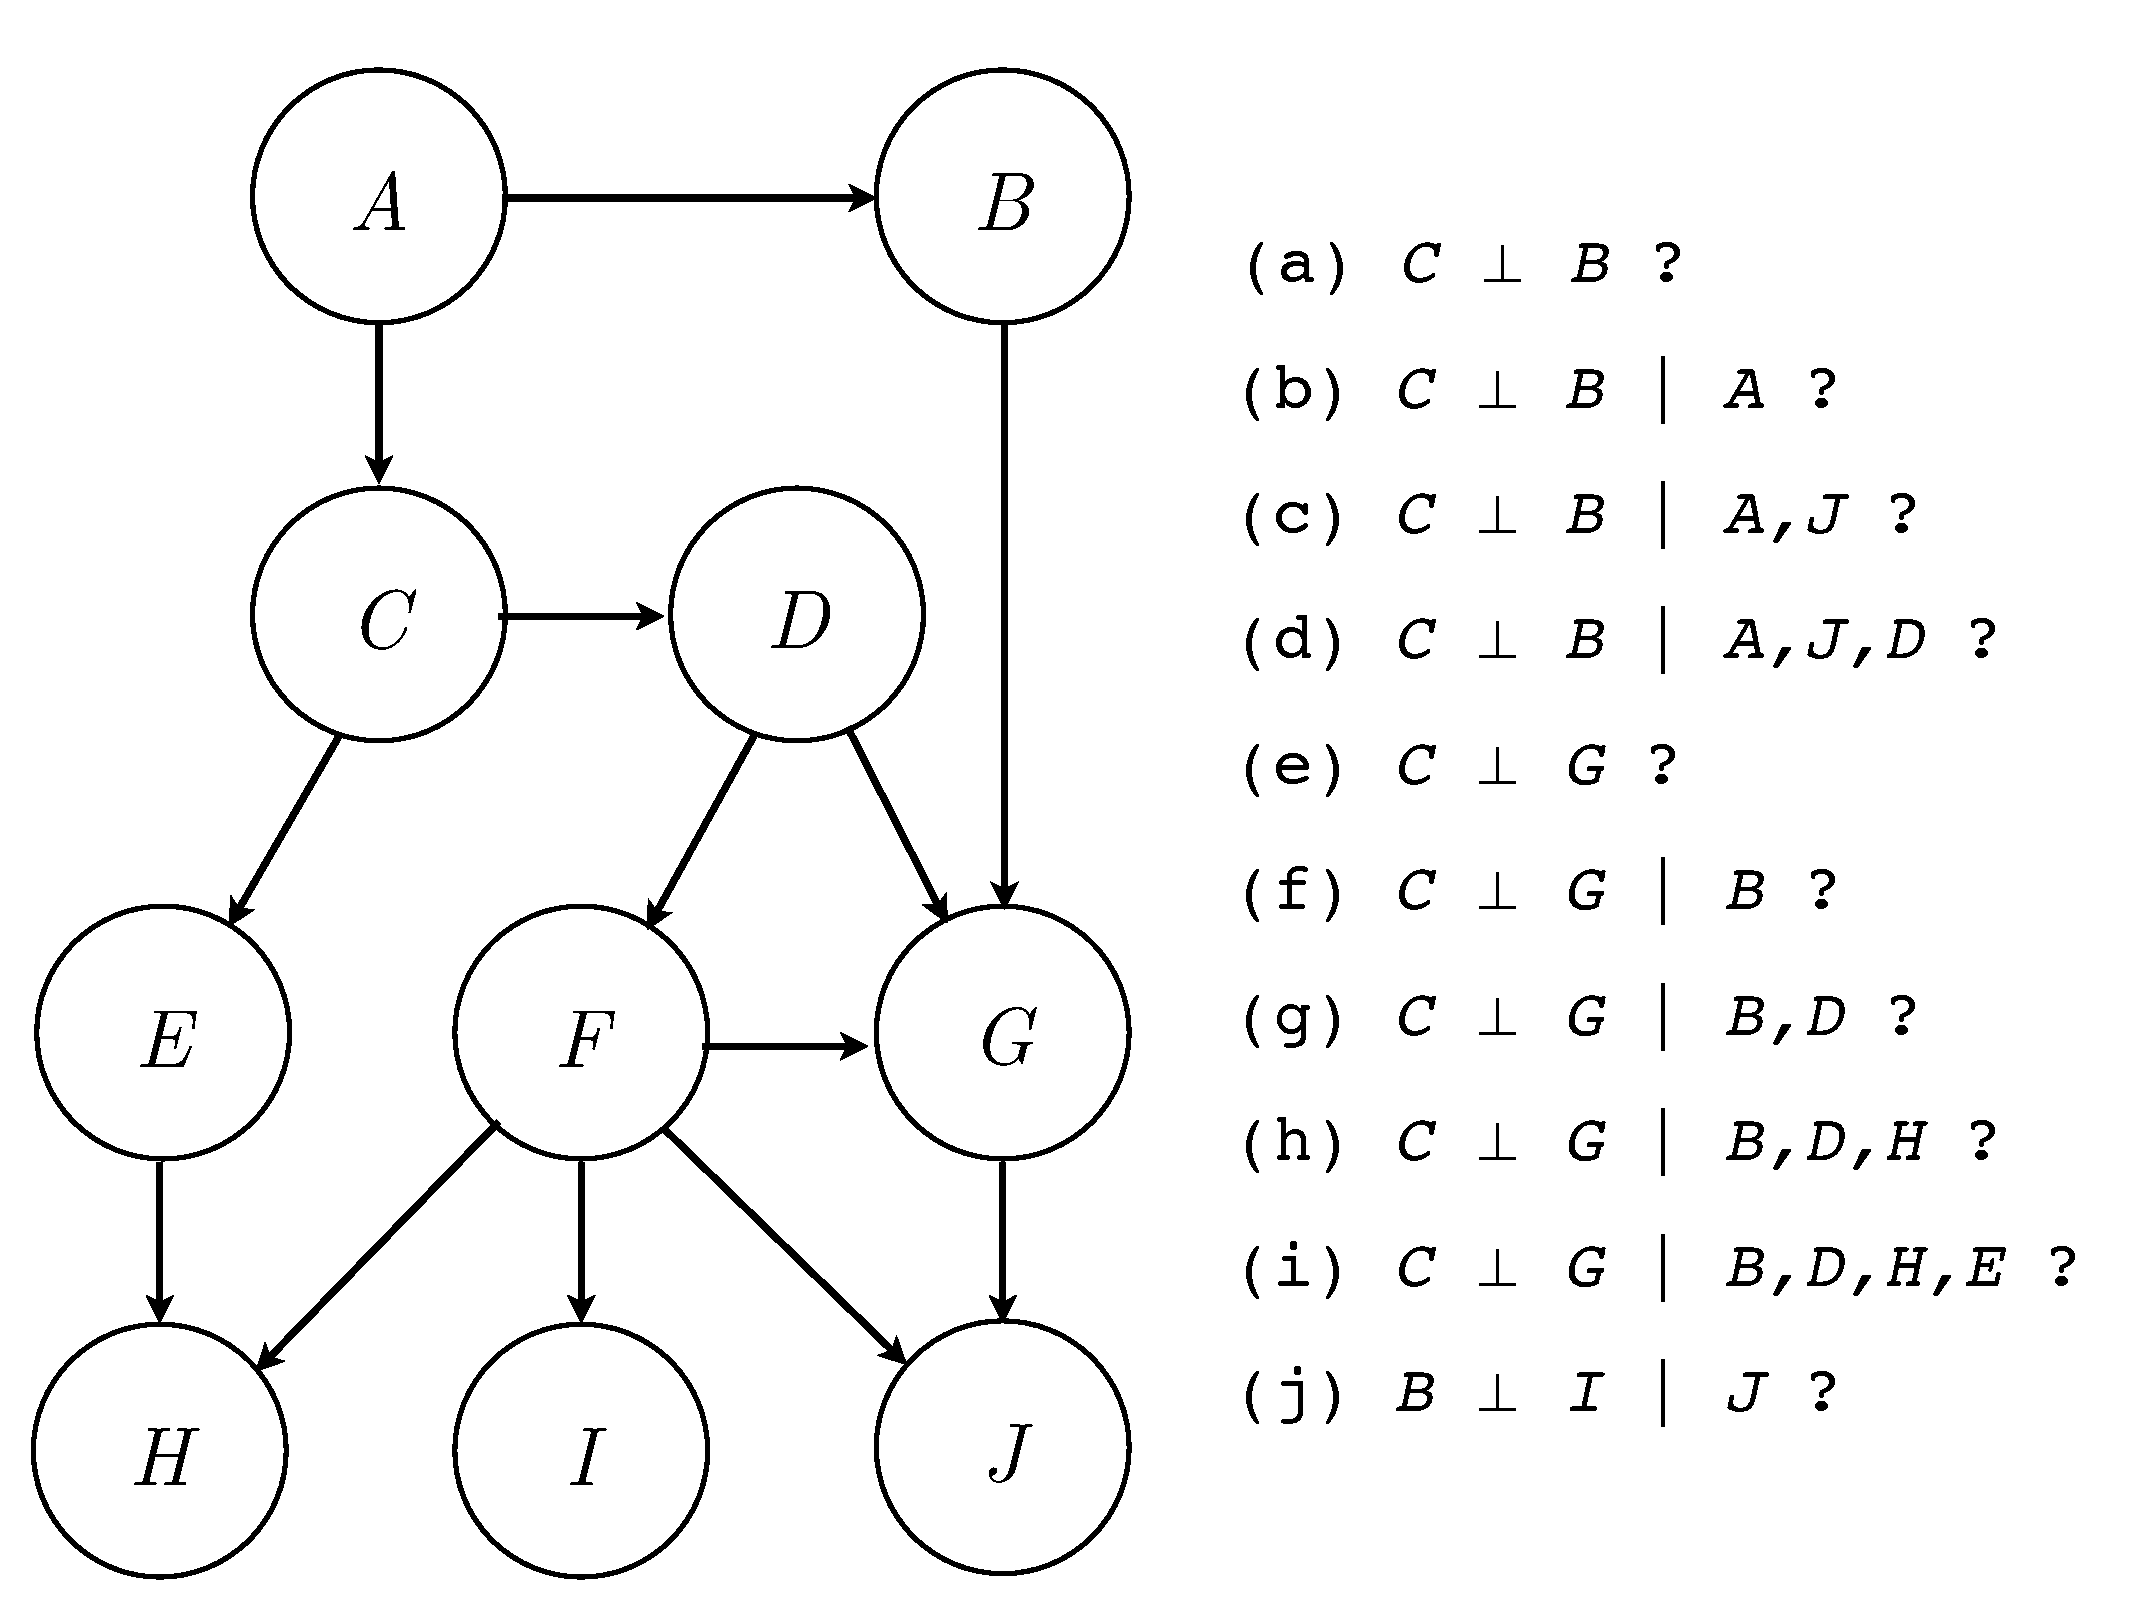
\includegraphics[scale=0.25]{hwk3_d-sep.pdf}
\end{center}

%--------------------
%    Question 3
%--------------------
% Get them to show the calculations for this question!!! 
% Assume p(x) = p(y) = 0.5
\item {\bf Positive interactions in-V-structure (10 points) } \\
Let $X, Y, Z$ be binary random variables with a joint
distribution parametrized according to the graph: $X \rightarrow Z
\leftarrow Y$. We define the following: 
\begin{equation}
\alpha := P(X = 1), \quad \beta := P (X = 1 \mid Z = 1), \quad  \gamma := P (X = 1 \mid Z
= 1, Y = 1) \nonumber
\end{equation}
\begin{enumerate}
\item For all the following cases, provide examples of joint
probability tables (and calculate the quantities $a$, $b$, $c$),
so that each of the following conditions are (individually) true: 
\begin{enumerate}[(i)]
\item $\gamma < \alpha$
\item $\alpha < \gamma < \beta$
\item $\beta < \alpha < \gamma$.
\end{enumerate}


\item Think of $X$ and $Y$ as causes and $Z$ as a common effect, for the previous three cases, briefly state (in a sentence or two) why the claims are true for your examples.
\end{enumerate}

Please use the following format to represent the joint distributions you choose for the cases in part \textit{a)}. Study the expected format carefully and note how this is sufficient to represent the joint distribution. Also, use the corresponding boxes to write the values of $\alpha$, $\beta$ and $\gamma$ for each of the three sub-questions.

\begin{center}

    \begin{tabular}{|c|c|c|}
        \hline
        $X$ & $Y$ & $P(X,Y)$ \\
        \hline
        1 & 1 &  \\
        \hline
        1 & 0 &  \\
        \hline
        0 & 1 &  \\
        \hline
        0 & 0 &  \\
        \hline
    \end{tabular}
    \hspace{5mm}
    \begin{tabular}{|c|c|c|}
        \hline
        $X$ & $Y$ & $P(Z=1 | X,Y)$ \\
        \hline
        1 & 1 &  \\
        \hline
        1 & 0 &  \\
        \hline
        0 & 1 &  \\
        \hline
        0 & 0 &  \\
        \hline
    \end{tabular}
    \hspace{5mm}
    \begin{tabular}{|c|c|c|}
        \hline
        $\alpha$ & $\beta$ & $\gamma$ \\
        \hline
        \hspace{9mm} & \hspace{9mm} & \hspace{9mm} \\
        \hline
    \end{tabular}
\end{center}


%--------------------
%    Question
%--------------------
\item {\bf Equivalence of directed tree DGM with undirected tree UGM (10 points) } \\
Let $G$ be a directed tree and $G'$ its corresponding undirected tree, i.e., the orientation of edges is ignored. Prove that $\mathcal{L}(G)=\mathcal{L}(G')$. \textit{Hint: Recall that by the definition of a directed tree, $G$ does not contain any v-structure.}

\vspace{0.2cm}

%--------------------
%    Question
%--------------------
\item {\bf Hammersley-Clifford counter-example (10 points)} \\
In class, we mentioned that the strict positivity of the joint distribution was crucial in the Hammersley-Clifford theorem. Here is a counter-example (4.4 in Koller \& Friedman) that shows the problems when we have zero probabilities.

Consider a joint distribution~$p$ over four binary random variables: $X_1$, $X_2$, $X_3$ and $X_4$ which gives probability
$\frac{1}{8}$ to each of the following eight configurations, and
zero to all others:
$$(0,0,0,0) \hspace{3mm} (1,0,0,0) \hspace{3mm} (1,1,0,0) \hspace{3mm} (1,1,1,0) \hspace{3mm} (0,0,0,1) \hspace{3mm} (0,0,1,1) \hspace{3mm} (0,1,1,1) \hspace{3mm} (1,1,1,1)$$

Let $G$ be the usual four nodes undirected graph
$X_{1}\text{---}X_{2}\text{---}X_{3}\text{---}X_{4}\text{---}X_{1}$. One can show that $p$ satisfies the 
global Markov property with respect to this graph $G$ because of trivial deterministic relationships. For example, if we condition on $X_2 = 0$ and $X_4=0$, then the only value of $X_3$ with non-zero probability is $X_3 = 0$, and thus $X_3 | (X_2=0 ,X_4=0)$ being a deterministic random variable, it is trivially conditionally independent to $X_1$. By (painfully) going through all other possibilities, we get similar situations: $X_2=0$ and $X_4=1$ forces $X_1 = 0$, etc. 

Prove that the distribution $p$ \textbf{cannot} factorize according to $G$, and thus $p \notin \mathcal{L}(G)$. \emph{Hint:} argue by contradiction.

%--------------------
%    Question
%--------------------
\item {\bf Bizarre conditional independence properties (10 BONUS points)} \\ 
Let $(X,Y,Z)$ be a random vector with a finite sample space. Consider the following statement: 
\begin{center}
``If  $X \indep Y \mid Z$ and $X \indep Y$ then ($X \indep Z$ or $Y \indep Z$).''
\end{center}
\BNUM
\item Is this true if one assumes that $Z$ is a binary variable? Prove or disprove.
\item Is the statement true in general? Prove or disprove.
\ENUM 


\item {\bf EM and Gaussian mixtures (4 points)}

Derive the form of the \textbf{M-step updates} for the parameters $\{\pi_k, \boldsymbol{\mu}_k, \sigma_k\}_{k=1}^K$ of a Gaussian mixture model in which the covariance matrices are proportional to the identity:
$$p(x) = \sum_{k=1}^K \pi_k \, \, \mathcal{N}(x \, | \, \boldsymbol{\mu}_k, \sigma_k \mathbf{I} )$$


\item {\bf Implementation: EM and Gaussian mixtures (26 points)} \\

Follow the instructions in this Colab notebook:

\url{https://colab.research.google.com/drive/1mtyFbcWZAuoNV8zBicoH1Y0Bc_Sv2c7G}


\end{enumerate}

\end{document}


